\section{Định nghĩa: đặc tính của dữ liệu hướng thời gian}
Phần này bao gồm các khía cạnh chính để mô tả thời gian và dữ liệu hướng thời gian. Điều quan trọng là phải phân biệt rõ giữa thời gian vật lý và mô hình thời gian trong các hệ thống thông tin. Khi mô hình hóa thời gian trong các hệ thống thông tin, mục tiêu không phải là bắt chước hoàn toàn thời gian vật lý, tuy nhiên để cung cấp mô hình phù hợp nhất để phản ánh các hiện tượng đang được xem xét và hỗ trợ các bài toán phân tích (bằng tay). Hơn nữa, theo Frank [132], không có mô hình đúng duy nhất, có nhiều cách để mô hình hóa thời gian trong các hệ thống thông tin và thời gian cũng được mô hình hóa trong các ứng dụng khác nhau phụ thuộc vào từng bài toán. Các nghiên cứu sâu rộng đã được tiến hành để hình thành khái niệm về thời gian trong nhiều lĩnh vực của khoa học máy tính bảo gồm cả trí tuệ nhân tạo, khai phá dữ liệu, mô phỏng, mô hình, cơ sở dữ liệu ... Chúng tôi phỏng theo các nghiên cứu của Frank [132] và Goralwalla et al [154], trong đó các khía cạnh trực giao chính được trình bày để mô tả các khía cạnh khác nhau của các loại thời gian. Dữ liệu cơ bản được trình bày trong chương 2, chúng tôi tập trung vào các đặc tính của thời gian và dữ liệu hướng thời gian nói riêng. Những khía cạnh này sẽ được mô tả chi tiết sau đây.
\subsection{Các đặc tính của thời gian}
Các đặc tính của thời gian có thể được chia thành các khía cạnh chung yêu cầu mô hình thời gian đầy đủ cũng như tổ chức phân cấp của thời gian và định nghĩa các yêu tố cụ thể. Các khía cạnh tổng quát bao gồm \textit{thang đo}, \textit{phạm vi}, \textit{sắp xếp} và \textit{góc nhìn}.
\begin{itemize}
    \item \textit{Thang đo}: \textit{thứ tự}, \textit{rời rạc}, \textit{liên tục}. Ở góc độ thứ nhất, chúng tôi xem xét thời gian theo thang đo dọc mà các thành phần của mô hình đã được cho trước. Trong miền thời gian theo \textit{thứ tự}, chỉ có quan hệ thứ tự tương đối được biểu diễn (ví dụ như: trước, sau, trong). Trong miền \textit{rời rạc}, khoảng thời gian cũng được xem xét. Các giá trị thời gian có thể được ánh xạ tới một tập các số nguyên, cho phép lập mô hình định lượng các giá trị thời gian. Miền thời gian rời rạc dựa trên đơn vị (ví dụ: giây, phút). Mô hình thời gian \textit{liên tục} đặc trưng bởi ánh xạ đến các số thực. Nghĩa là giữa hai mốc thời gian, tồn tại một mốc thời gian khác (cũng có thể hiểu là mô hình mật độ thời gian).
    \item \textit{Phạm vi}: dựa trên \textit{thời điểm}, dựa trên \textit{khoảng}. Chúng tôi xem xét phạm vi của các yếu tố cơ bản cấu thành nên miền thời gian. Thời gian dựa trên \textit{thời điểm} có thể được biểu diễn như các điểm Euclide rời rạc trong không gian, tức là có mốc thời gian bằng 0. Như vậy không có thông tin được đưa về khoảng giữa 2 thời điểm. Trái ngược với đó, miền dựa theo \textit{khoảng} có độ lớn lớn hơn 0. Khái niệm này cũng có liên quan chặt chẽ đến khái niệm về độ chi tiết, sẽ được bàn luận sau. Ví dụ, giá trị thời gian ngày 1/5/2014 có thể liên quan đến một thời điểm riêng lẻ là 2014-05-01 00:00:00 là một điểm theo miền dựa trên \textit{thời điểm} cũng có thể là đoạn [2014-05-01 00:00:00, 2014-05-01 23:59:99] trong miền dựa trên \textit{khoảng}
    \item \textit{Sắp xếp}: \textit{tuyến tính}, \textit{tuần hoàn}. Tương tự với nhận thức tự nhiên, chúng ta coi thời gian là một quá trình \textit{tuyến tính} từ quá khứ đến tương lai, tức là mỗi giá trị thời gian có một giá trị duy nhất ở hiện tại cũng như tương lai. Trong cách sắp xếp \textit{tuần hoàn} thời gian được xem xét theo các giá trị định kì (ví dụ mùa trong năm).
    \item \textit{Góc nhìn}: \textit{thứ tự}, \textit{nhánh}, \textit{đa góc nhìn}. Miền thời gian theo \textit{thứ tự} xem xét sự kiện xảy ra sau sự kiện khác. Chi tiết hơn, chúng ta cũng có thể phân biệt giữa thứ tự toàn phần và thứ tự một phần. Trong miền thứ tự toàn phần, chỉ một sự kiện có thể xảy ra trong một thời điểm. Trái với đó, các sự kiện đồng thời hoặc chồng chéo được cho phép trong miền thứ tự một phần. Một dạng phức tạp hơn của mô hình thời gian được gọi là \textit{nhánh} thời gian. Trong mô hình này, nhiều nhánh của thời gian có thể được mô tả với các kịch bản khác nhau (ví dụ mô hình lập kế hoạch). Trái ngược với thời gian phân nhánh, chỉ có một đường thực sự diễn ra theo thời gian, mô hình \textit{đa góc nhìn} cho phép nhiều phương án xảy ra đồng thời theo thời gian. Ví dụ nhiều nhân chứng mô tả cùng một tình huống, mỗi người có một góc nhìn khác nhau và kể một câu chuyện khác nhau.
\end{itemize}
Phân loại thứ bậc thời gian và các yếu tố thời gian cụ thể được xác định dựa trên độ chi tiết, đơn vị thời gian và tính xác định.
\begin{itemize}
    \item \textit{Độ chi tiết và lịch}: \textit{rỗng}, \textit{đơn} và \textit{nhiều}. Để giải quyết độ phức tạp về thời gian và đưa ra các độ chi tiết khác nhau, chúng ta có thể sử dụng vài giải thích vắn tắt hữu ích. Về cơ bản \textit{độ chi tiết} là một khái niệm trừu tượng về thời gian (do chúng ta tự định nghĩa) để hình dung thời gian một cách dễ dàng hơn trong cuộc sống (chẳng hạn như giờ, phút, giây). Tổng quan hơn, độ chi tiết mô tả ánh xạ từ thời gian đến các đơn vị nhỏ hơn hoặc lớn hơn. Nếu độ chi tiết và hệ thống lịch được hỗ trợ bởi mô hình thời gian, chúng tôi mô tả nó như \textit{nhiều} chi tiết. Bên cạnh biến thể phức tạp này, có thể chỉ có một \textit{đơn} chi tiết hoặc là \textit{không} có khái niệm trừu tượng nào trong này được hỗ trợ.
    \item \textit{Nguyên thủy thời gian}: \textit{tức thời}, \textit{khoảng thời gian}, \textit{nhịp}. Những nguyên thủy thời gian này có thể được xem như một lớp trung gian giữa các phần tử dữ liệu và miền thời gian. Về cơ bản, thời gian nguyên thủy có thể được chia thành neo nguyên thủy (tuyệt đối) và không neo (tương đối). \textit{tức thời} và \textit{khoảng thời gian} thuộc nhóm đầu tiên, tức là chúng nằm trên một ví trí cố định trên miền thời gian. Ngược lại, một \textit{nhịp} là một tính chất tương đối, tức là nó không có vị trí tuyệt đối trên miền thời gian. Tức thời là mô hình dành cho các điểm riêng lẻ trên trục thời gian (đôi khi còn gọi là thời điểm, ví dụ 10/5/2014), khoảng thời gian là khoảng giữa hai thời điểm (ví dụ từ 10/5/2014 đến 16/5/2014), nhịp là thời lượng (của khoảng) mà không có mốc cố định (ví dụ 6 ngày).
    \item \textit{Tính xác định}: \textit{xác định}, \textit{không xác định}. Sự không chắc chắn là một khía cạnh quan trọng khác cần được xem xét của dữ liệu hướng thời gian. Nếu không có thông tin đầy đủ hay chính xác về thời gian hoặc nếu thời gian gốc được chuyển đổi từ độ chi tiết này sang độ chi tiết khác thì sự không chắc chắn sẽ xuất hiện và cần được xử lý. Ví dụ cho điều này là sự không chính xác đến từ kiến thức thực tế (ví dụ thời điểm trái đất hình thành), các dữ liệu được lập kế hoạch trong tương lai (ví dụ nhiệm vụ cần khoảng 2 đến 3 tháng để hoàn thành) hoặc là các sự kiện không chắc chắn (ví dụ khoảng 2 đến 3 ngày trước). Lưu ý rằng tính không xác định thời gian cũng như tính tương đối của các tham chiếu đến thời gian chủ yếu là các tiêu chuẩn của các phát biểu hơn là các sự kiện mà chúng biểu thị. Tính không xác định có thể được hiểu bởi các thông số rõ ràng (ví dụ bắt đầu sớm nhất và bắt đầu gần nhất của một khoảng thời gian) hoặc ngầm hiểu trong trường hợp đa độ chi tiết nhỏ. Ví dụ, xem xét một câu khẳng định "Hoạt động A bắt đầu vào ngày 14 tháng 5 năm 2014 và kết thúc vào ngày 17 tháng 5 năm 2014" - khẳng định này có thể được mô hình hóa bằng điểm bắt đầu "14/5/2014" và điểm kết thúc "17/5/2014" cả hai đều có độ chi tiết tính đến ngày. Nếu ta nhìn vào khoảng này với độ chi tiết theo giờ, khoảng có thể bắt đầu và kết thúc vào các điểm giữa 0 AM và 12 PM của một ngày nhất định. Chính vì vậy, \textit{tính xác đinh} của tham số thời gian cho trước cần phần được phân tích. Một thông số được biểu diễn khi có kiến thức đầy đủ về  tất cả các khía cạnh của thời gian.
\end{itemize}
Trong phần tiếp theo, chúng tôi khám phá và xác định dữ liệu hướng thời gian một cách chi tiết hơn.
\subsection{Các đặc tính của dữ liệu hướng thời gian}
Cũng như các tính chất của thời gian, dữ liệu có tác động lớn đến việc thiết kế phương pháp trực quan hóa. Chúng ta cùng lược qua những yếu tố chính của dữ liệu liên quan đến thời gian.
\begin{itemize}
    \item \textit{Quy mô}: \textit{định tính}, \textit{định lượng}. Dữ liệu định lượng được dựa trên một thang đo (rời rạc hoặc liên tục). Dữ liệu định tính mô tả tập hợp các phần tử dữ liệu có thứ thự hoặc không có thứ tự.
    \item \textit{Hệ quy chiếu}: \textit{trừu tượng}, \textit{không gian}. Dữ liệu trừu tượng (ví dụ tài khoản ngân hàng) được thu thập trong bối cảnh phi không gian. Dữ liệu không gian (ví dụ dữ liệu điều tra dân số) chứa thông tin về không gian ví dụ như vị trí địa lý.
    \item \textit{Loại dữ liệu}: \textit{sự kiện}, \textit{trạng thái}. Sự kiện có thể được hiểu là các điểm đánh dấu sự thay đổi trạng thái (ví dụ sự khời hành của đoàn tàu), trong khi đó trạng thái đặc trưng cho các giai đoạn liên tục giữa các sự kiện (ví dụ đoàn tàu đang chạy trên đường sắt).
    \item \textit{Số biến}: \textit{đơn biến}, \textit{đa biến}. Dữ liệu đơn biến chỉ chứa một giá trị dữ liệu tại một thời điểm, trong trường hợp đa biến, dữ liệu tại mỗi thời điểm thể hiện bằng nhiều giá trị dữ liệu.
\end{itemize}
Những phạm trù cơ bản này tạo thành cơ sở cho việc lựa chọn, thiết lập kĩ thuật trực quan hóa phù hợp cho dữ liệu hướng thời gian. 
\subsection{Dữ liệu liên quan và thời gian}
Các khía cạnh liên quan của dữ liệu phụ thuộc vào thời gian đã được kiểm tra rộng rãi trong lĩnh vực cơ sở dữ liệu về thời gian [274,397]. Ở đây, chúng tôi điều chỉnh và phát triển các định nghĩa trong lĩnh vực này. Theo đó, bất kì tập dữ liệu nào cũng có liên quan đến 2 miền thời gian: (1) thời gian bên trong và (2) thời gian bên ngoài. 
\\ \\
\textit{Thời gian bên trong} được coi là chiều thời gian vốn có của mô hình dữ liệu. Thời gian bên trong mô tả thời điểm thông tin tồn tại trong tập dữ liệu là hợp lệ. Ngược lại \textit{thời ian bên ngoài} là thời gian nằm ngoài mô hình dữ liệu. Thời gian bên ngoài là cần thiết để mô tả cách một tập dữ liệu phát triển theo thời gian. Dựa vào số biến thời gian nguyên thủy của thời gian bên trong và thời gian bên ngoài, dữ liệu liên quan đến thời gian có thể được phân loại như sau:
\begin{itemize}
    \item \textit{Dữ liệu tĩnh phi thời gian}. Nếu cả thời gian bên trong lẫn bên ngoài bao gồm một yếu tố thời gian thì dữ liệu hoàn toàn không phụ thuộc vào thời gian. Trong chương này chúng ta sẽ không kiểu dữ liệu đó.
    \item \textit{Dữ liệu thời gian tĩnh}. Nếu thời gian bên trong chứa nhiều hơn một yếu tố thời gian nguyên thủy, trong khi thời gian bên ngoài chỉ chứa một thì dữ liệu có thể được xem là phụ thuộc vào thời gian. Vì các giá trị được lưu trong dữ liệu phụ thuộc vào thời gian bên trong , dữ liệu thời gian tĩnh có thể được hiểu là một cái nhìn lịch sử về cách một số mô hình xem xét các yếu tố khác nhau của thời gian trong. Chuỗi thời gian chung là một ví dụ tiêu biểu về dữ liệu thời gian tĩnh. 
    \item \textit{Dữ liệu động phi thời gian}. Nếu thời gian bên trong chỉ chứa một mà thời gian bên ngoài chứa nhiều yếu tố thời gian nguyên thủy thì dữ liệu phụ thuộc vào thời gian bên ngoài. Để cho dễ hiểu, dữ liệu thay đổi qua thời gian thì chúng được gọi là động. Vì thời gian bên trong không được xem xét nên chỉ có trạng thái hiện tại của dữ liệu là bảo toàn. Cái nhìn quá khứ không được duy trì ở đây nữa. Có vài kĩ thuật trực quan hóa sẵn có tập trung vào dữ liệu động phi thời gian, tuy nhiên do thời gian bên trong và thời gian bên ngoài có thể ánh xạ lẫn nhau, một số kĩ thuật trực quan hóa cho dữ liệu tĩnh cũng có thể áp dụng được.
    \item \textit{Dữ liệu động theo thời gian}. Nếu cả thời gian bên trong và bên ngoài đều có nhiều yếu tố thời gian nguyên thủy, thì dữ liệu được xem xét là phụ thuộc vào thời gian. Nói cách khác, dữ liệu chứa các biến phụ thuộc vào thời gian (bên trong) và trạng thái dữ liệu cũng thay đổi theo thời gian (bên ngoài). Thường thì trong trường hợp này, thời gian bên trong và bên ngoài phụ thuộc lẫn nhau và có thể ánh xạ vào nhau. Sự phân biệt rõ ràng giữa thời gian bên trong và bên ngoài thường không được thực hiện bởi các phương pháp trực quan hóa hiện tại bởi xem xét cả 2 chiều thời gian để trực quan hóa là một thách thức.
\end{itemize}
\begin{figure}[H] % places figure environment here   
    \centering % Centers Graphic
    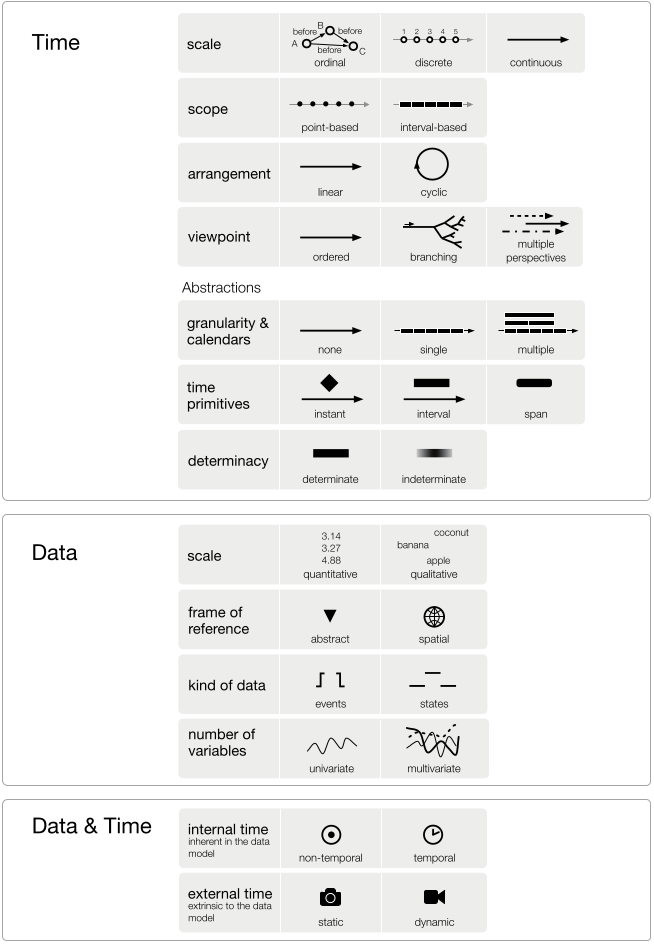
\includegraphics[width=0.9\textwidth]{assets/fig_7_2.png} 
    \caption{Các khía cạnh của dữ liệu hướng thời gian} % Creates caption underneath graph
    \label{fig:fig7.2}
\end{figure}